\documentclass{beamer}
% \usepackage[utf8]{inputenc}

\usepackage{amsmath, amsfonts, amssymb}
\usepackage{amsthm}
\usepackage{mathtools}
\usepackage{physics}
\usepackage[super]{nth}

\usepackage{graphicx}
\graphicspath{{../assets/}}

\usepackage{pgfplots}
\usepackage{tikz}
\usepackage{standalone}

\usepackage[english]{isodate}

\newcommand{\ee}{\operatorname{e}}          % Euler's number
\newcommand{\ii}{\mathrm{i}}                % imaginary unit
\newcommand{\ad}[1]{a_{#1}^{\dagger}}       % creation operator
\newcommand*\mean[1]{\overline{#1}}         % mean

\usetheme[progressbar=frametitle]{metropolis}           % Use metropolis theme
\usepackage{appendixnumberbeamer}

\title{Large-Scale Numerical Investigations into the Dynamics of Nonlinear Classical Systems}
\subtitle{SIAM Conference on Applications of Dynamical Systems}
\date{Snowbird, 22 \printdayoff\today}
\author{Sebastian Micluța-Câmpeanu}
\institute{University of Bucharest}

\begin{document}
\maketitle%

%%%%%%%%%%%%%%%%%%%%%%%%%%%% slide 1 %%%%%%%%%%%%%%%%%%%%%%%%%%%%

\begin{frame}{Outline}
  \tableofcontents[]
\end{frame}

%%%%%%%%%%%%%%%%%%%%%%%%%%%% slide 2 %%%%%%%%%%%%%%%%%%%%%%%%%%%%

\begin{frame}{Acknowledgements}
	\begin{itemize}
		\item I would like to thank A.I.~Nicolin, and V.~Băran for helping and motivating me.
		\item The author has been	supported by the research project PN-III-P4-ID-PCE-2016-0792
		funded by the Romanian Minisrty of Research and Inovation.
		\item All numerical simulations were performed on the computing cluster of
		Department of Computational Physics and Information Technologies,
		``Horia Hulubei'' National Institute for Physics and Nuclear Engineering.
	\end{itemize}
\end{frame}

\section{Introduction}

%%%%%%%%%%%%%%%%%%%%%%%%%%%% slide 3 %%%%%%%%%%%%%%%%%%%%%%%%%%%%

\begin{frame}{The model}
  \begin{itemize}
		\item The physical system that we model \cite{micluta-campeanu2018} is the surface of heavy nuclei.
    \item We use a Hamiltonian that describes the constrained
		motion of the vibrational quadrupole degrees of freedom of
		the nuclear surface.
  \end{itemize}
\end{frame}

%%%%%%%%%%%%%%%%%%%%%%%%%%%% slide 4 %%%%%%%%%%%%%%%%%%%%%%%%%%%%

\begin{frame}{The model}
	The Hamiltonian of the system
	\begin{equation*}
    H = \alert<1,2>{\frac{A}{2}\left(p_0^2+p_2^2\right)+\frac{A}{2}\left(q_0^2+q_2^2\right)}
		 +\alert<3>{\frac{B}{\sqrt{2}}q_0\left(3q_2^2-q_0^2\right)}
		 +\alert<2>{\frac{D}{4}\left(q_0^2+q_2^2\right)^2}
  \end{equation*}

	\begin{columns}
		\column{0.5\textwidth}
		\begin{itemize}
			\item \alert<1> {Harmonic oscillator part}
			\item \alert<2> {Integrable part}
			\item \alert<3> {Non-integrable term}
		\end{itemize}

		\column{0.5\textwidth}
		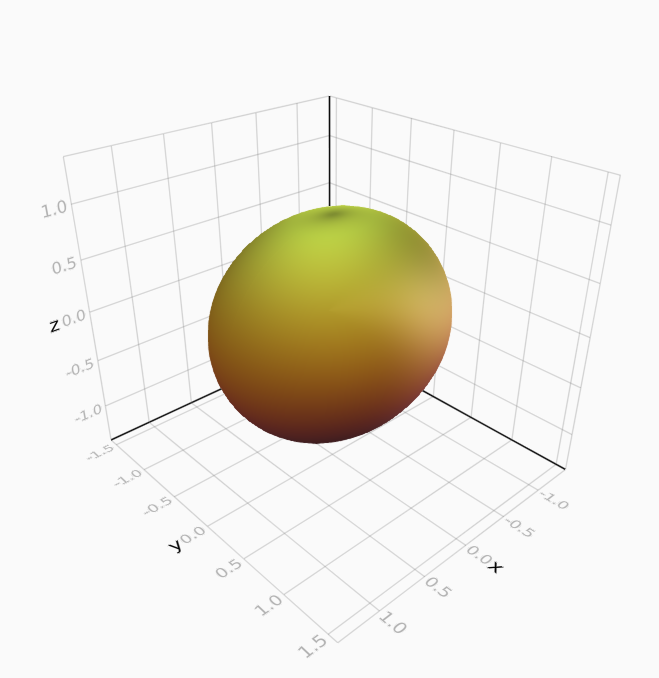
\includegraphics[width=\textwidth]{nucleus}
	\end{columns}
\end{frame}

%%%%%%%%%%%%%%%%%%%%%%%%%%%% slide 5 %%%%%%%%%%%%%%%%%%%%%%%%%%%%

\begin{frame}
	\begin{figure}
		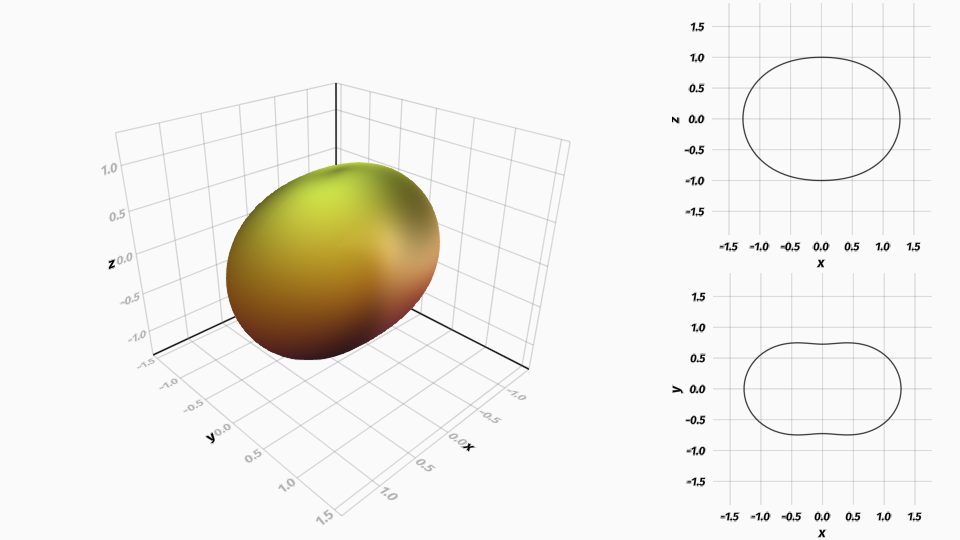
\includegraphics[width=\textwidth]{nucleus-with-sections}
		\caption{The nuclear surface and its sections}
	\end{figure}
\end{frame}

%%%%%%%%%%%%%%%%%%%%%%%%%%%% slide 6 %%%%%%%%%%%%%%%%%%%%%%%%%%%%

\begin{frame}
	\begin{figure}
		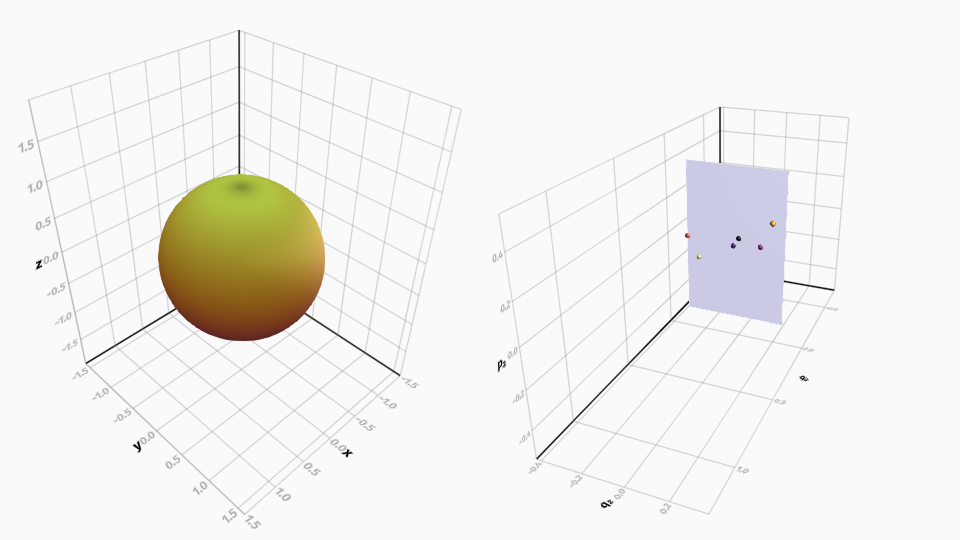
\includegraphics[width=\textwidth]{nucleus-with-poincare}
		\caption{The nucleus and the corresponding trajectory in the phase space
		for a chaotic trajectory with \(B=0.5, E=0.3\)}
	\end{figure}
\end{frame}

\section{Numerical simulations}

\subsubsection{Using the \texttt{Julia} ecosystem}

%%%%%%%%%%%%%%%%%%%%%%%%%%%% slide 7 %%%%%%%%%%%%%%%%%%%%%%%%%%%%

\begin{frame}{\texttt{Julia}}
	\begin{itemize}
		\item Numerical simulations and the visualizations of the
		results was done in \texttt{Julia} \cite{Julia-2017} (\texttt{DifferentialEquations.jl} \cite{DifferentialEquations.jl-2017}
		and \texttt{DynamicalSystems.jl} \cite{DynamicalSystems.jl-2018} for simulations and respectively
		\texttt{Plots.jl} and \texttt{Makie.jl} for visualizations).
		\item Having access to the implementations of a large
		number of integrators helps us taking an informed decision
		for the choiche of the integration algorithm.
	\end{itemize}
\end{frame}

%%%%%%%%%%%%%%%%%%%%%%%%%%%% slide 8 %%%%%%%%%%%%%%%%%%%%%%%%%%%%

\begin{frame}
	\begin{figure}
		\includestandalone[width=\textwidth]{../assets/short-benchmark-E}
		\caption{Energy error benchmark for short integration time}
	\end{figure}
\end{frame}

%%%%%%%%%%%%%%%%%%%%%%%%%%%% slide 9 %%%%%%%%%%%%%%%%%%%%%%%%%%%%

\begin{frame}
	\begin{figure}
		\includestandalone[width=\textwidth]{../assets/short-benchmark-t}
		\caption{Computational time benchmark for short integration time}
	\end{figure}
\end{frame}

%%%%%%%%%%%%%%%%%%%%%%%%%%%% slide 10 %%%%%%%%%%%%%%%%%%%%%%%%%%%%

\begin{frame}
	\begin{figure}
		\includestandalone[width=\textwidth]{../assets/long-benchmark-E}
		\caption{Energy error benchmark for long integration time}
	\end{figure}
\end{frame}

%%%%%%%%%%%%%%%%%%%%%%%%%%%% slide 11 %%%%%%%%%%%%%%%%%%%%%%%%%%%%

\begin{frame}
	\begin{figure}
		\includestandalone[width=\textwidth]{../assets/long-benchmark-t}
		\caption{Computational time benchmark for long integration time}
	\end{figure}
\end{frame}

\subsubsection{The maximal Lyapunov exponent}

%%%%%%%%%%%%%%%%%%%%%%%%%%%% slide 12 %%%%%%%%%%%%%%%%%%%%%%%%%%%%

\begin{frame}{Quantifying chaoticity}
	\begin{itemize}
		\item The maximal Lyapunov exponent is defined as
		\[
			\lambda = \lim\limits_{t \to \infty} \frac{1}{t} \ln{\frac{\dd{x}(t)}{\dd{x}(0)}}
		\]
		\item One of the signature characheristics of chaos is the sensitivity to the initial conditions	(\(\lambda > 0\)).
		\item We can get some intuitive insight for the sensitivity to
		the initial conditions by following the evolution of two nearby
		initial conditions.
	\end{itemize}
\end{frame}


%%%%%%%%%%%%%%%%%%%%%%%%%%%% slide 13 %%%%%%%%%%%%%%%%%%%%%%%%%%%%

\begin{frame}
	\begin{figure}
		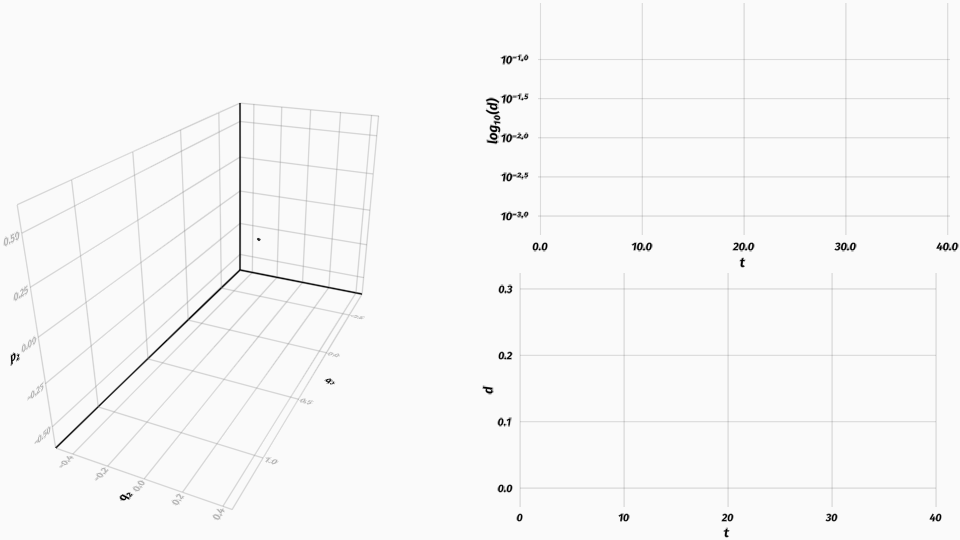
\includegraphics[width=\textwidth]{dist-with-log}
		\caption{The distance between nearby trajectories for \(B=0.5\)
		and \(E=0.3\).}
	\end{figure}
\end{frame}

%%%%%%%%%%%%%%%%%%%%%%%%%%%% slide 14 %%%%%%%%%%%%%%%%%%%%%%%%%%%%

\begin{frame}{Interactive exploratinos}
	\begin{itemize}
		\item For a given set of parameters ($B$ and $E$) we have
		a set of compatible initial conditions.
		\item Poincaré sections give us a global picture of the
		dynamics.
		\item For a better (visual) understanding of the dynamics
		we can show the Lyapunov exponents on the Poincaré map.
	\end{itemize}
\end{frame}

%%%%%%%%%%%%%%%%%%%%%%%%%%%% slide 15 %%%%%%%%%%%%%%%%%%%%%%%%%%%%

\begin{frame}
	\begin{figure}
		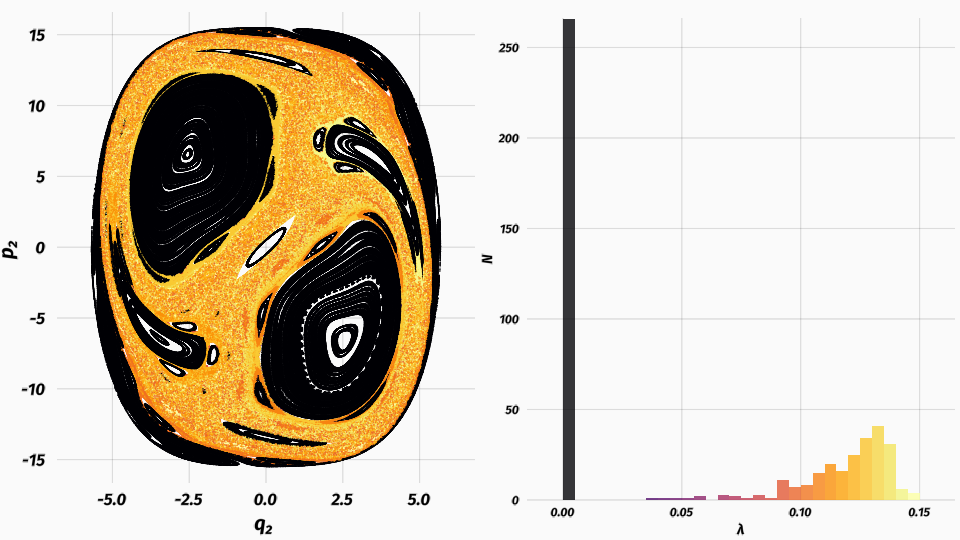
\includegraphics[width=\textwidth]{poincare}
		\caption{A Poincaré section at \(B=0.5, E=120\)}
	\end{figure}
\end{frame}

%%%%%%%%%%%%%%%%%%%%%%%%%%%% slide 16 %%%%%%%%%%%%%%%%%%%%%%%%%%%%

\begin{frame}{A note regarding the \(\lambda\) histogram}
	\begin{itemize}
		\item Theoretically the Lyapunov exponent histogram should
		have two sharp peaks: one for the regular part and one for
		the chaotic one.
		\item The spread in the chaotic part is given by finite time
		effects.
		\item To better understand this we will take a look at how
		the integration time affects the results.
	\end{itemize}
\end{frame}

%%%%%%%%%%%%%%%%%%%%%%%%%%%% slide 17 %%%%%%%%%%%%%%%%%%%%%%%%%%%%

\begin{frame}
	\begin{figure}
		\includestandalone[width=\textwidth]{../assets/hist-lambda-4}
		\caption{Maximal Lyapunov coefficient histogram for \(B=0.5\)
		and \(E=120\).}
	\end{figure}
\end{frame}

%%%%%%%%%%%%%%%%%%%%%%%%%%%% slide 18 %%%%%%%%%%%%%%%%%%%%%%%%%%%%

\begin{frame}
	\begin{figure}
		\includestandalone[width=\textwidth]{../assets/hist-lambda-5}
		\caption{Maximal Lyapunov coefficient histogram for \(B=0.5\)
		and \(E=120\).}
	\end{figure}
\end{frame}

%%%%%%%%%%%%%%%%%%%%%%%%%%%% slide 19 %%%%%%%%%%%%%%%%%%%%%%%%%%%%

\begin{frame}
	\begin{figure}
		\includestandalone[width=\textwidth]{../assets/hist-lambda-6}
		\caption{Maximal Lyapunov coefficient histogram for \(B=0.5\)
		and \(E=120\).}
	\end{figure}
\end{frame}

%%%%%%%%%%%%%%%%%%%%%%%%%%%% slide 20 %%%%%%%%%%%%%%%%%%%%%%%%%%%%

\begin{frame}
	\begin{figure}
		\includestandalone[width=\textwidth]{../assets/hist-lambda-7}
		\caption{Maximal Lyapunov coefficient histogram for \(B=0.5\)
		and \(E=120\).}
	\end{figure}
\end{frame}

%%%%%%%%%%%%%%%%%%%%%%%%%%%% slide 21 %%%%%%%%%%%%%%%%%%%%%%%%%%%%

\begin{frame}{Averaging \(\lambda\) over the initial conditions}
	\begin{itemize}
		\item We define the averaged Lyapunov coefficient as the
		mean of the maximal Lyapunov exponents in the chaotic region.
		\item We need a sufficiently robust method of selecting
		the \(\lambda\)s in the chaotic region.
		\item We consider as chaotic everything after the first
		local maxima in the histogram.
	\end{itemize}
\end{frame}

%%%%%%%%%%%%%%%%%%%%%%%%%%%% slide 22 %%%%%%%%%%%%%%%%%%%%%%%%%%%%

\begin{frame}
	\begin{figure}
		\includestandalone[width=\textwidth]{../assets/hist-lambda-selected-before}
		\caption{Selecting the chaotic trajectories for \(B=0.5\)
		and \(E=120\).}
	\end{figure}
\end{frame}

%%%%%%%%%%%%%%%%%%%%%%%%%%%% slide 23 %%%%%%%%%%%%%%%%%%%%%%%%%%%%

\begin{frame}
	\begin{figure}
		\includestandalone[width=\textwidth]{../assets/hist-lambda-selected-after}
		\caption{Selecting the chaotic trajectories for \(B=0.5\)
		and \(E=120\).}
	\end{figure}
\end{frame}

%%%%%%%%%%%%%%%%%%%%%%%%%%%% slide 24 %%%%%%%%%%%%%%%%%%%%%%%%%%%%

\begin{frame}
	\begin{figure}
		\includestandalone[width=\textwidth]{../assets/mean-over-ic}
		\caption{Averaged \(\lambda\) for \(B=0.5\) and \(E \in (10, 3000)\).}
	\end{figure}
\end{frame}

%%%%%%%%%%%%%%%%%%%%%%%%%%%% slide 25 %%%%%%%%%%%%%%%%%%%%%%%%%%%%

\begin{frame}
	\begin{figure}
		\includestandalone[width=\textwidth]{../assets/mean-over-ic-low}
		\caption{Averaged \(\lambda\) for \(B=0.5\) and \(E \in (0.01, 10)\).}
	\end{figure}
\end{frame}

%%%%%%%%%%%%%%%%%%%%%%%%%%%% slide 26 %%%%%%%%%%%%%%%%%%%%%%%%%%%%

\begin{frame}{Other indicators}
	\begin{itemize}
		\item We can look at the distance between two nearby
		trajectories in the limit of \(T \to \infty\) in order to
		get an estimate of the phase space volume. We will denote this as
		\(d_\infty\).
		\item In a finite phase space volume we cannot have only an
		exponential divergence of trajectories, so there must be some
		something that folds the trajectories back after the initial
		divergence\cite{baranFolding2015}.
		\item We define \(\Gamma\) as a measure of folding
		\[
		\Gamma = \frac{\ee^\lambda - 1}{d_\infty}
		\]
		\item We can apply similar averaging techniques as for \(\lambda\).

	\end{itemize}
\end{frame}

%%%%%%%%%%%%%%%%%%%%%%%%%%%% slide 27 %%%%%%%%%%%%%%%%%%%%%%%%%%%%

\begin{frame}
	\begin{figure}
		\includestandalone[width=\textwidth]{../assets/mean-over-ic-dinf}
		\caption{Averaged \(d_\infty\) for \(B=0.5\) and \(E \in (0.01, 10)\).}
	\end{figure}
\end{frame}

%%%%%%%%%%%%%%%%%%%%%%%%%%%% slide 28 %%%%%%%%%%%%%%%%%%%%%%%%%%%%

\begin{frame}
	\begin{figure}
		\includestandalone[width=\textwidth]{../assets/mean-over-ic-Gamma}
		\caption{Averaged \(\Gamma\) for \(B=0.5\) and \(E \in (0.01, 10)\).}
	\end{figure}
\end{frame}

%%%%%%%%%%%%%%%%%%%%%%%%%%%% slide 29 %%%%%%%%%%%%%%%%%%%%%%%%%%%%

\begin{frame}{Averaging \(\lambda\) over the energy}
	\begin{itemize}
		\item We can get a global picture of the sistem by integrating
		the averaged Lyapunov coefficient over an energy interval.
		\item For a small energy interval in the low energy limit we
		get a monotonusly increasing dependence.
		\item For a large energy interval we have a non-trivial
		dependence of the averaged Lyapunov exponent with respect
		to the non-integrability parameter $B$.
	\end{itemize}
\end{frame}

%%%%%%%%%%%%%%%%%%%%%%%%%%%% slide 30 %%%%%%%%%%%%%%%%%%%%%%%%%%%%

\begin{frame}
	\begin{figure}
		\includestandalone[width=\textwidth]{../assets/mean-over-E-low}
		\caption{Averaged \(\lambda\) for \(B=0.5, E \in (10, 3000)\)
		and \(B \in (0.1, 0.6)\).}
	\end{figure}
\end{frame}

%%%%%%%%%%%%%%%%%%%%%%%%%%%% slide 31 %%%%%%%%%%%%%%%%%%%%%%%%%%%%

\begin{frame}
	\begin{figure}
		\includestandalone[width=\textwidth]{../assets/mean-over-E}
		\caption{Averaged \(\lambda\) for \(B=0.5, E \in (0.01, 10)\)
		and \(B \in (0.1, 0.6)\).}
	\end{figure}
\end{frame}

%%%%%%%%%%%%%%%%%%%%%%%%%%%% slide 32 %%%%%%%%%%%%%%%%%%%%%%%%%%%%

\section{Conclusions}

\begin{frame}{Conclusions}
	\begin{itemize}
		\item The \texttt{Julia} ecosystem provides performant and
		flexible tools for exploring dynamical systems.
		\item We investigated in detail the classical dynamics of a
		non-integrable system and found a series of interesting
		phenomena with respect to its phase-space structure as
		function of energy and the non-integrability parameter.
		\item In order to propote open and reproducible\cite{singularity-2017,white2018datadepsjl} science the presentation and the dataset needed for the visualizations
		are freely available online at \url{https://github.com/SebastianM-C/DS19Presentation}.
	\end{itemize}
\end{frame}

%%%%%%%%%%%%%%%%%%%%%%%%%%%% slide 33 %%%%%%%%%%%%%%%%%%%%%%%%%%%%

\begin{frame}[allowframebreaks]{References}

  \bibliography{reference}
  \bibliographystyle{abbrv}

\end{frame}

%%%%%%%%%%%%%%%%%%%%%%%%%%%% slide 27 %%%%%%%%%%%%%%%%%%%%%%%%%%%%

\begin{frame}[standout]
Thank you!
\end{frame}

\appendix

%%%%%%%%%%%%%%%%%%%%%%%%%%%% slide a1 %%%%%%%%%%%%%%%%%%%%%%%%%%%%

\begin{frame}
	\begin{figure}
		\includestandalone[width=\textwidth]{../assets/potential-contour}
		\caption{The equipotential lines for \(V\) at \(B=0.5\).}
	\end{figure}
\end{frame}

%%%%%%%%%%%%%%%%%%%%%%%%%%%% slide a2 %%%%%%%%%%%%%%%%%%%%%%%%%%%%

\begin{frame}
	\begin{figure}
		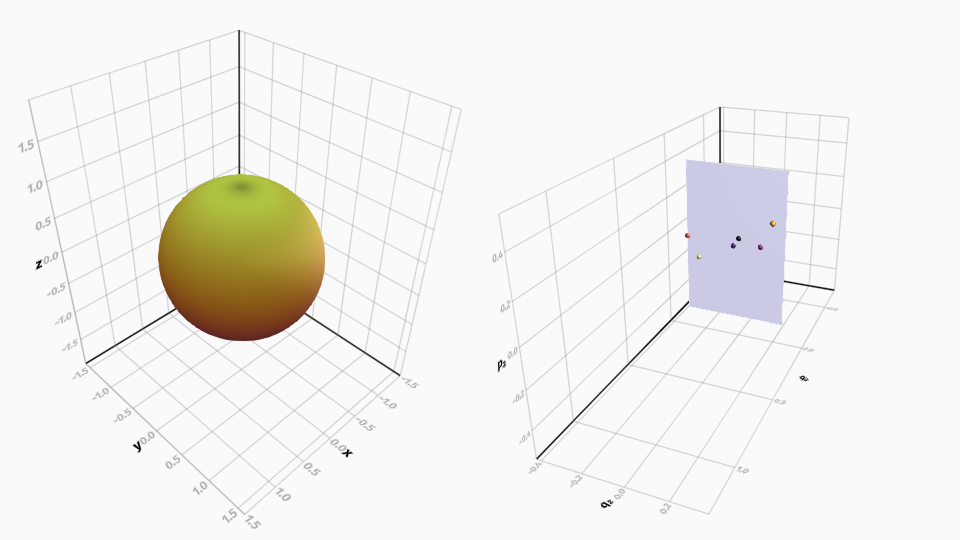
\includegraphics[width=\textwidth]{nucleus-with-poincare}
		\caption{The nucleus and the corresponding trajectory in the phase space
		for a regular trajectory with \(B=0.5, E=0.3\)}
	\end{figure}
\end{frame}

%%%%%%%%%%%%%%%%%%%%%%%%%%%% slide a3 %%%%%%%%%%%%%%%%%%%%%%%%%%%%

\begin{frame}
	\begin{figure}
		\includestandalone[width=\textwidth]{../assets/short-benchmark-rescaling-E}
		\caption{Energy error benchmark for short integration time with rescaling}
	\end{figure}
\end{frame}

%%%%%%%%%%%%%%%%%%%%%%%%%%%% slide a4 %%%%%%%%%%%%%%%%%%%%%%%%%%%%

\begin{frame}
	\begin{figure}
		\includestandalone[width=\textwidth]{../assets/short-benchmark-rescaling-t}
		\caption{Computational time benchmark for short integration time with rescaling}
	\end{figure}
\end{frame}

%%%%%%%%%%%%%%%%%%%%%%%%%%%% slide a5 %%%%%%%%%%%%%%%%%%%%%%%%%%%%

\begin{frame}
	\begin{figure}
		\includestandalone[width=\textwidth]{../assets/long-benchmark-rescaling-E}
		\caption{Energy error benchmark for long integration time with rescaling}
	\end{figure}
\end{frame}

%%%%%%%%%%%%%%%%%%%%%%%%%%%% slide a6 %%%%%%%%%%%%%%%%%%%%%%%%%%%%

\begin{frame}
	\begin{figure}
		\includestandalone[width=\textwidth]{../assets/long-benchmark-rescaling-t}
		\caption{Computational time benchmark for long integration time with rescaling}
	\end{figure}
\end{frame}

%%%%%%%%%%%%%%%%%%%%%%%%%%%% slide a7 %%%%%%%%%%%%%%%%%%%%%%%%%%%%

\begin{frame}
	\begin{figure}
		\includestandalone[width=\textwidth]{../assets/mean-over-ic-T-comparison}
		\caption{Averaged \(\lambda\) for \(B=0.5\) and \(E \in (10, 3000)\).}
	\end{figure}
\end{frame}

%%%%%%%%%%%%%%%%%%%%%%%%%%%% slide a8 %%%%%%%%%%%%%%%%%%%%%%%%%%%%

\begin{frame}
	\begin{figure}
		\includestandalone[width=\textwidth]{../assets/mean-over-ic-B-difference}
		\caption{Averaged \(\lambda\) for \(B \in {0.5,0.6}\) and \(E \in (10, 3000)\).}
	\end{figure}
\end{frame}

\end{document}
